\section{Methods used}

\begin{frame}[c]{Grafeno sintezės reakcijos simuliacijos įrankis}
    \begin{figure}
        \centering
        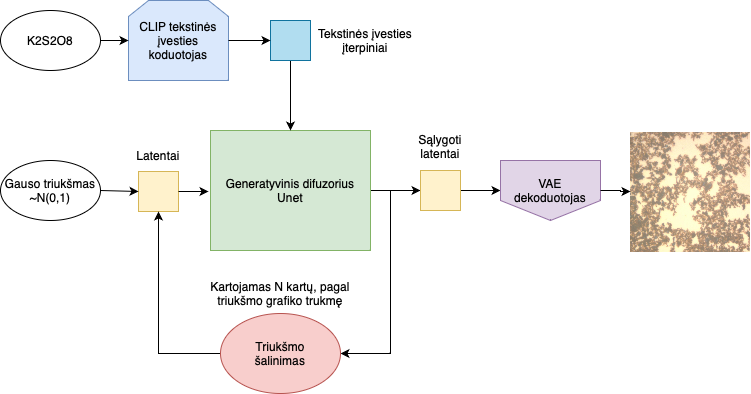
\includegraphics[width=0.75\textwidth]{img/text2image_grafenas_gulscias.png}
        \caption{Grafeno sintezės reakcijos simuliacijos įrankio architektūra \cite{LatentDiffusion}}
        \label{fig:text2image_pipeline}
    \end{figure}
\end{frame}

\begin{frame}[c]{CLIP mokymas}
    \begin{figure}
        \centering
        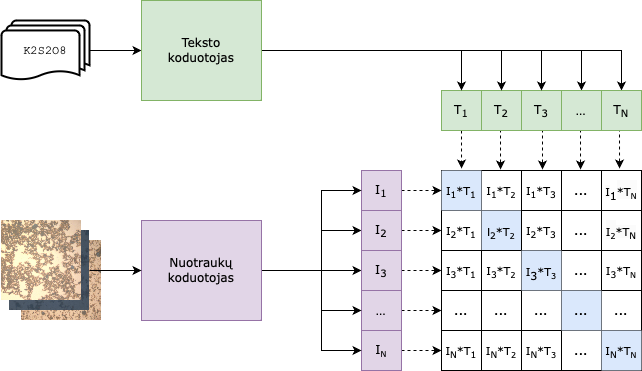
\includegraphics[width=0.6\textwidth]{img/CLIP_training_lt.png}
        \caption{CLIP mokymas}
        \label{fig:clip_training}
    \end{figure}
    \begin{center}
        {\tiny \cite{CLIP}}
    \end{center}
\end{frame}

\begin{frame}[c]{CLIP naudojimas}
    \begin{figure}
        \centering
        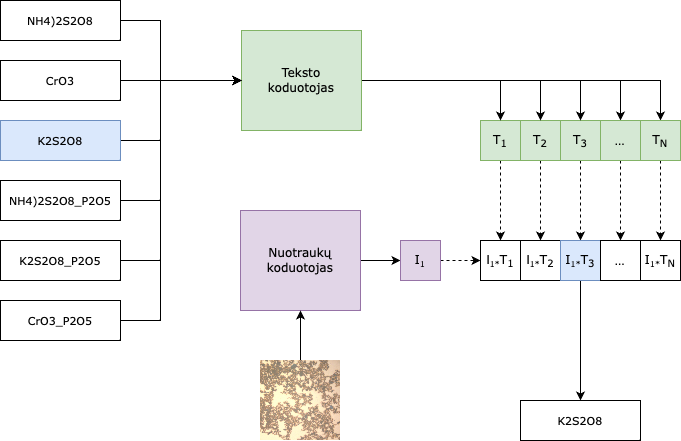
\includegraphics[width=0.58\textwidth]{img/CLIP_inference_lt.png}
        \caption{CLIP naudojimas}
        \label{fig:clip_inference}
    \end{figure}
    \begin{center}
        {\tiny \cite{CLIP}}
    \end{center}
\end{frame}



\begin{frame}[c]{Generatyvinis difuzijos modelis}
    \begin{equation}
        q(x_{1:T}|x_0) := \prod_{t=1}^{T}q(x_t|x_{t-1}), \quad\quad q(x_t|x_{t-1}) := \mathcal{N}(x_t| \sqrt{1 - \beta_t}x_{t-1}, \beta_t\textbf{I}) \label{eq:diffusion_process}
    \end{equation}
    \begin{equation}
        p_\theta(x_{0:T}) := p(x_T)\prod_{t=1}^{T}p_\theta(x_{t-1}|x_t), \quad\quad p_\theta(x_{t-1}|x_t) := \mathcal{N}(x_{t-1}| \boldsymbol{\mu}_\theta(x_t, t), \boldsymbol{\Sigma}_\theta(x_t, t))
        \label{eq:reverse_process}
    \end{equation}
    \begin{center}
        {\tiny \cite{Diffusion_Ho}}
    \end{center}
    \begin{figure}
        \centering
        
\includegraphics[width=0.8\textwidth]{img/Markov_Chain.png}
        \caption{Difuzijos procesas}
        \label{fig:diffusion}
    \end{figure}
\end{frame}
